%%%%%%%%%%%%%%%%%%%%%%%%%%%%%%%%%%%%%%%%%%%%%%%%%%%
%% P3: Phenomenology of Particle Physics                         
%%
%% Author:  André Rubbia                   		 
%%
%% Figure 2.12 Collinear and head-on collisions of particle $1$ crossing a region containing particles of type $2$.
%%
%% This work is licensed under the Creative Commons Attribution 4.0 International License. 
%% To view a copy of this license, visit http://creativecommons.org/licenses/by/4.0/ or 
%% send a letter to Creative Commons, PO Box 1866, Mountain View, CA 94042, USA.
%%
%%%%%%%%%%%%%%%%%%%%%%%%%%%%%%%%%%%%%%%%%%%%%%%%%%%

\documentclass[a4paper,10pt]{article}

\usepackage[T1]{fontenc}
\usepackage[utf8]{inputenc}
\usepackage{lmodern}
\usepackage[labelfont=bf]{caption}
\usepackage{upgreek}
\usepackage{amssymb}
\usepackage{amsmath}

\usepackage{tikz}
\usepackage{pgfplots}
\pgfplotsset{compat=1.17}
\usepgfplotslibrary{ternary}
\usepgfplotslibrary{fillbetween}
\usepgfplotslibrary{external}

\def\d{\mathrm{d}}

\begin{document}

%%%%%%%%%%%%%%%   FIGURE  %%%%%%%%%%%%%%%%%%%%%%%%%%%%%%
\begin{figure}[htb]
\begin{center}
    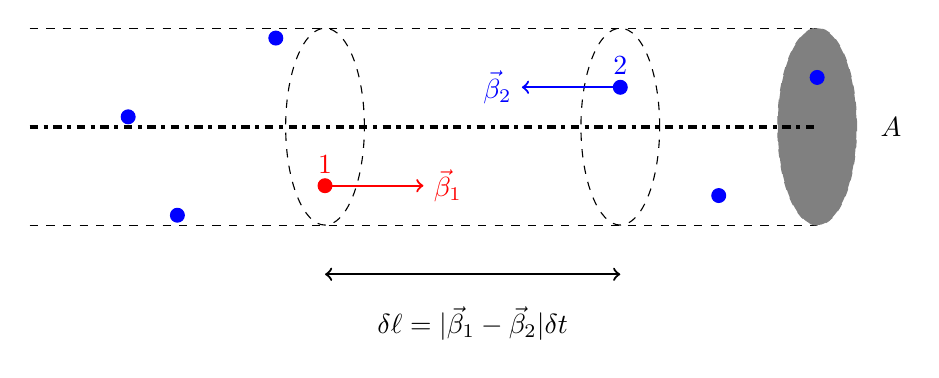
\begin{tikzpicture}[scale=1.25]
         \draw[dashed] (-3,0) -- (5,0);
         \draw[dashed] (-3,2) -- (5,2);
         \filldraw[gray,dashed]  (5,1) ellipse (0.4 and 1);
         \draw[dashed]  (0,1) ellipse (0.4 and 1);
         \draw[dashed]  (3,1) ellipse (0.4 and 1);
         \draw[line width=1.5, dash dot] (-3,1) -- (5,1);
         \filldraw [red] (0,0.4) circle (2pt) node[above=1pt] {1};
         \draw[red,thick,->] (0,0.4) -- +(0:1) node[right] {$\vec \beta_1$};
         \filldraw [blue] (3,1.4) circle (2pt) node[above=1pt] {2};
         \filldraw [blue] (-2,1.1) circle (2pt);
         \filldraw [blue] (4,0.3) circle (2pt);
         \filldraw [blue] (-1.5,0.1) circle (2pt);
         \filldraw [blue] (5,1.5) circle (2pt);
         \filldraw [blue] (-0.5,1.9) circle (2pt);
        \draw[blue,thick,->] (3,1.4) -- +(-180:1) node[left] {$\vec \beta_2$};
        \draw[black,thick,<->] (0,-0.5) -- (3,-0.5);
        \node at (1.5,-1) {$\delta \ell = \vert\vec \beta_1-\vec\beta_2\vert\delta t$};
        \node at (5.75,1.) {$A$};
  \end{tikzpicture}
\caption{Collinear and head-on collisions of particle $1$ crossing a region containing particles of type $2$.}
\end{center}
\end{figure}
%%%%%%%%%%%%%%%   END FIGURE  %%%%%%%%%%%%%%%%%%%%%%%%%%%%%%%

\end{document}
